\chapter{Tổng quan về hệ thống}
\label{chap:overview-system}

\section{Ý tưởng thiết kế hệ thống}
MiniClaw vận hành theo mô hình trợ lý ảo chạy nền (daemon) ưu tiên cục bộ (local-first). Hệ thống sử dụng thư viện Grammy làm giao diện Telegram Bot nhằm tiếp nhận yêu cầu lập lịch trình, quản lý công việc và tương tác hội thoại tự nhiên. Song song đó, giao diện dòng lệnh (CLI) cho phép nhà phát triển cấu hình trực tiếp tiến trình daemon.

Hình \ref{fig:miniclaw-interaction-model} minh họa tổng quan luồng tương tác và kiến trúc phân tầng của hệ thống.

\begin{figure}[H]
  \centering
  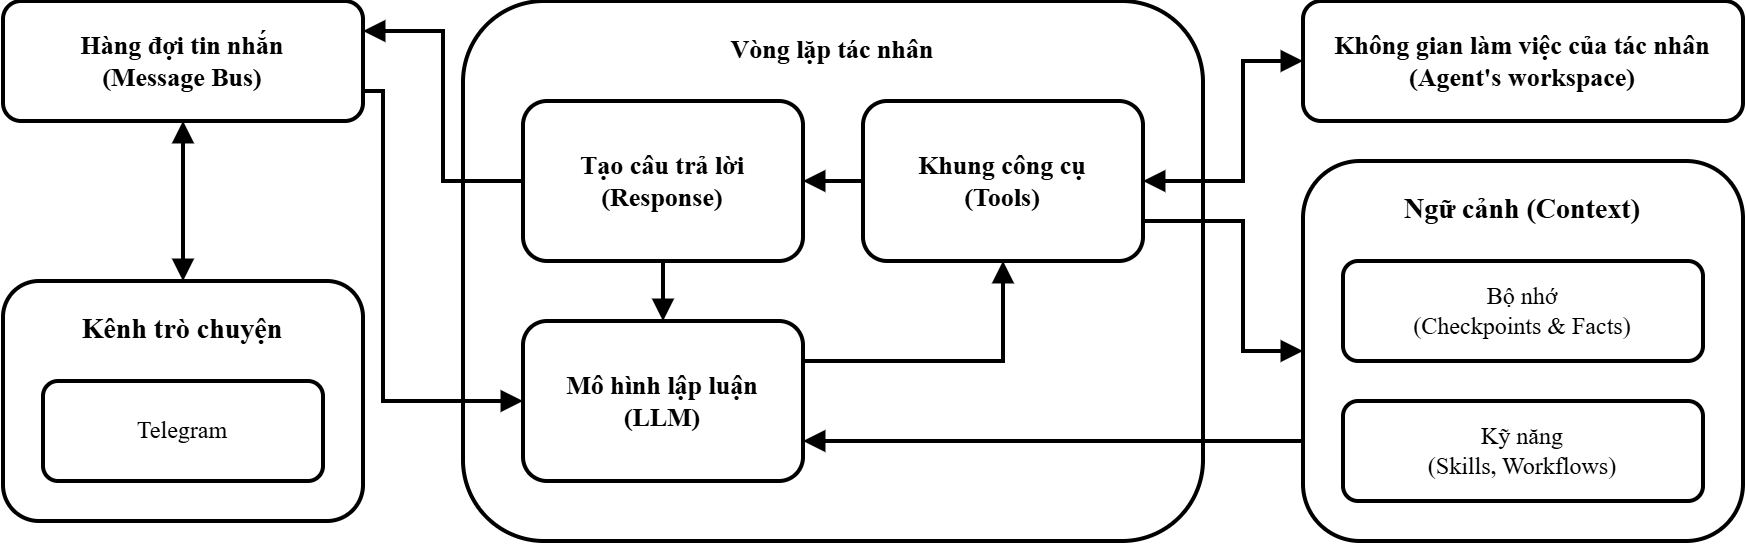
\includegraphics[width=0.9\linewidth]{figures/architecture_overview.drawio}
  \caption[\emph{Sơ đồ phân tầng tương tác MiniClaw.}]{\emph{Sơ đồ phân tầng cấu trúc tương tác của hệ thống MiniClaw.}}
  \label{fig:miniclaw-interaction-model}
\end{figure}

Phân tích sơ đồ Hình \ref{fig:miniclaw-interaction-model} cho thấy quyết định thiết kế phân tách rõ ranh giới bảo mật (security boundary) ngay tại máy chủ cá nhân. Cấu trúc này giữ toàn bộ thông tin nhạy cảm (lịch trình, bộ nhớ ngắn hạn) ở môi trường cục bộ, chặn đứng rủi ro rò rỉ dữ liệu. Cơ chế chuyển đổi dự phòng (fallback) giữa mô hình Ollama (cục bộ) và API đám mây thương mại đảm bảo cân bằng giữa tính riêng tư, hiệu năng suy luận và chi phí vận hành.

\section{Các nguyên tắc thiết kế cốt lõi}

\subsection{Xử lý bất đồng bộ và gộp tin nhắn (Message Coalescing)}
Người dùng Telegram thường có thói quen gửi liên tiếp nhiều tin nhắn ngắn. Nếu xử lý từng thông điệp độc lập, hệ thống sẽ kích hoạt vòng lặp tác nhân (agent loop) dồn dập, gây lãng phí tài nguyên suy luận. Nhằm cô lập tiến trình cốt lõi khỏi nhịp độ giao tiếp của client, tầng MessageBus triển khai cơ chế gộp tin nhắn (message coalescing). Các luồng sự kiện đến trong cửa sổ 250ms được gom thành một cụm dữ liệu (batch) duy nhất trước khi chuyển giao cho tác nhân.

Hình \ref{fig:message-coalescing-flow} mô tả chi tiết luồng gộp tin nhắn bất đồng bộ.

\begin{figure}[H]
  \centering
  % Tự động thu phóng toàn bộ sơ đồ vừa vặn với chiều ngang trang A4 (\textwidth)
  \resizebox{\textwidth}{!}{
  \begin{tikzpicture}[
      every node/.style={font=\small},
      header/.style={rectangle, draw=black!80, fill=black!5, thick, rounded corners=2pt, minimum height=0.9cm, align=center, font=\small\bfseries},
      active/.style={rectangle, fill=gray!15, draw=black!70, thick},
      msg/.style={thick, ->, >=stealth, font=\scriptsize},
      reply/.style={thick, dashed, ->, >=stealth, font=\scriptsize},
      % Tăng inner sep từ 5pt lên 8pt để chữ trong hộp note thoải mái hơn
      note/.style={rectangle, draw=blue!50, fill=blue!5, rounded corners=2pt, align=left, inner sep=8pt, font=\scriptsize, thick}
  ]
    
    % 1. Vẽ Headers định vị tương đối (Không dùng tọa độ X cứng)
    % Khoảng cách node=2.5cm tự động giãn đều các thành phần
    \node[header] (user) {Người dùng\\(Telegram User)};
    \node[header, right=2.5cm of user] (tg) {Telegram Bot\\(Grammy Channel)};
    \node[header, right=2.5cm of tg] (bus) {MessageBus\\(Inbound Queue)};
    \node[header, right=2.5cm of bus] (loop) {AgentLoop\\(LangGraph)};

    % Định nghĩa biến Y trục dọc để dễ điều chỉnh độ cao tổng (Giãn từ -8.5 xuống -11.5)
    \def\bottomY{-11.5}

    % 2. Vẽ Lifelines tự động kéo từ Header xuống đáy
    \draw[dashed, gray!80, thick] (user) -- (user |- 0,\bottomY);
    \draw[dashed, gray!80, thick] (tg) -- (tg |- 0,\bottomY);
    \draw[dashed, gray!80, thick] (bus) -- (bus |- 0,\bottomY);
    \draw[dashed, gray!80, thick] (loop) -- (loop |- 0,\bottomY);

    % 3. Vẽ Activations bằng phép chiếu tọa độ (|-): Lấy X của header, Y tự chỉ định
    % Telegram Bot Activations (Điều chỉnh tọa độ Y giãn ra)
    \draw[active] ([xshift=-0.15cm]tg |- 0, -1.5) rectangle ([xshift=0.15cm]tg |- 0, -2.1);
    \draw[active] ([xshift=-0.15cm]tg |- 0, -4.2) rectangle ([xshift=0.15cm]tg |- 0, -4.8);
    \draw[active] ([xshift=-0.15cm]tg |- 0, -10.4) rectangle ([xshift=0.15cm]tg |- 0, -11.0);
    
    % MessageBus Activation
    \draw[active] ([xshift=-0.15cm]bus |- 0, -2.1) rectangle ([xshift=0.15cm]bus |- 0, -10.4);
    
    % AgentLoop Activation
    \draw[active] ([xshift=-0.15cm]loop |- 0, -8.0) rectangle ([xshift=0.15cm]loop |- 0, -9.8);

    % 4. Vẽ Message & Actions (Thêm above=4pt để chữ không dính vào đường line)
    
    % Giai đoạn 1: Tin nhắn M1
    \draw[msg] (user |- 0,-1.5) -- node[above=4pt] {1. Gửi M1 ("Hello")} ([xshift=-0.15cm]tg |- 0,-1.5);
    \draw[msg] ([xshift=0.15cm]tg |- 0,-2.1) -- node[above=4pt] {2. publishInbound(M1)} ([xshift=-0.15cm]bus |- 0,-2.1);
    \node[note, anchor=west] at ([xshift=0.3cm]bus |- 0,-2.9) {Khởi chạy bộ đếm\\thời gian 250ms (debounce)};
    
    % Giai đoạn 2: Tin nhắn M2 (Đến trong cửa sổ 250ms)
    \draw[msg] (user |- 0,-4.2) -- node[above=4pt] {3. Gửi M2 ("Cần giúp")} ([xshift=-0.15cm]tg |- 0,-4.2);
    \draw[msg] ([xshift=0.15cm]tg |- 0,-4.8) -- node[above=4pt] {4. publishInbound(M2)} ([xshift=-0.15cm]bus |- 0,-4.8);
    \node[note, anchor=west] at ([xshift=0.3cm]bus |- 0,-5.6) {Nhận M2 trong cửa sổ\\$\Rightarrow$ Reset timer 250ms};

    % Giai đoạn 3: Timeout & Gom cụm
    \node[note, anchor=east] at ([xshift=-0.3cm]bus |- 0,-6.8) {Timer hết giờ (Timeout)\\\textbf{Gom cụm (Coalesce)}\\M1 + M2 $\rightarrow$ 1 Batch};

    % Giai đoạn 4: Đẩy Batch cho AgentLoop xử lý
    \draw[msg] ([xshift=0.15cm]bus |- 0,-8.0) -- node[above=4pt] {5. consumeInboundBatch()} ([xshift=-0.15cm]loop |- 0,-8.0);
    
    % Self-loop tự động bám mép trái của AgentLoop (Thêm left=6pt cho text)
    \draw[msg] ([xshift=-0.15cm]loop |- 0,-8.4) -- ++(-1.0,0) |- node[pos=0.25, left=6pt, align=left, font=\scriptsize] {Thực thi Agent Loop\\(Reasoning \& Tool Calls)} ([xshift=-0.15cm]loop |- 0,-9.4);
    
    % Giai đoạn 5: Phản hồi
    \draw[reply] ([xshift=-0.15cm]loop |- 0,-9.8) -- node[below=4pt] {6. publishOutbound(Response)} ([xshift=0.15cm]bus |- 0,-9.8);
    \draw[msg] ([xshift=-0.15cm]bus |- 0,-10.4) -- node[above=4pt] {7. consumeOutbound()} ([xshift=0.15cm]tg |- 0,-10.4);
    \draw[msg] ([xshift=-0.15cm]tg |- 0,-11.0) -- node[above=4pt] {8. Phản hồi gộp (Consolidated Reply)} (user |- 0,-11.0);
    
  \end{tikzpicture}
  } % Kết thúc \resizebox
  \caption{\emph{Sơ đồ luồng gộp tin nhắn.}}
  \label{fig:message-coalescing-flow}
\end{figure}

Sơ đồ Hình \ref{fig:message-coalescing-flow} chỉ ra tính độc lập giữa luồng tiếp nhận API và luồng suy luận. Mặc dù tạo ra độ trễ nhân tạo 250ms, quyết định đánh đổi (trade-off) này giúp hệ thống hấp thụ các đợt tải đột biến (spike load) và duy trì tính toàn vẹn ngữ cảnh cho LLM.

\subsection{Tính bảo mật và ranh giới an toàn (Security Boundary)}
Nhằm ngăn chặn rủi ro thực thi mã độc do ảo giác mô hình (hallucination), kiến trúc hệ thống áp đặt ranh giới bảo mật nghiêm ngặt. Phân hệ kiểm soát thực thi đánh giá ranh giới đường dẫn an toàn (Safe Path Validation), giam lỏng (sandbox) quyền truy cập tệp tin của tác nhân trong thư mục làm việc định sẵn. Hệ thống duy trì một danh sách trắng (allow-list) các tệp thực thi ngoại vi, chỉ cấp quyền gọi các công cụ văn phòng an toàn như \texttt{gws} hoặc \texttt{lark-cli}.

\subsection{Nạp động quy trình làm việc (Dynamic Workflow Loading)}
Phân hệ quản lý kỹ năng (Skill Manager) quét và tự động nạp cấu hình từ các thư mục lưu trữ. Ngay khi người dùng phê duyệt qua cơ chế kiểm soát (HITL), hệ thống chuyển tệp Markdown sang không gian làm việc của tác nhân. Tiếp theo, module quản lý sẽ trích xuất phần miêu tả kỹ năng và luồng làm việc để nạp các quy trình mới này vào ngữ cảnh tác nhân. Thiết kế này giúp MiniClaw mở rộng năng lực thực thi tức thì và tránh phải khởi động lại tiến trình nền (daemon).

\section{Vòng lặp hoạt động chính của hệ thống}

\subsection{Vòng lặp tương tác chính (Agent Loop)}
Vòng lặp này xử lý luồng hội thoại trực tiếp, tra cứu thông tin bộ nhớ dài hạn và thực thi thao tác lịch trình. Động cơ điều phối LangGraph vận hành kiến trúc ReAct, buộc tác nhân phải tuần tự suy luận (reasoning) ý định người dùng trước khi gọi công cụ (acting) nhằm đảm bảo tính chính xác của phản hồi.

\subsection{Vòng lặp nhắc nhở (Scheduler Daemon)}
Bộ lập lịch nhắc nhở (Scheduler) vận hành độc lập với vòng lặp hội thoại. Phân hệ này liên tục giám sát trạng thái tệp dữ liệu không gian làm việc. Khi chạm mốc thời gian đã định, hệ thống tự động cập nhật trạng thái sự kiện thành \emph{fired}, đồng bộ log vào lịch sử ngữ cảnh ngắn hạn và đẩy trực tiếp thông điệp nhắc qua hàng đợi MessageBus đến thiết bị người dùng.

\subsection{Vòng lặp trích xuất quy trình làm việc (Extraction Loop)}
Phân hệ nén và trích xuất ngữ cảnh vận hành ngầm định kỳ dưới nền. Khi lượng token trong lịch sử hội thoại vượt ngưỡng cấu hình (mặc định 50.000 token), hệ thống kích hoạt luồng trích xuất. Tác nhân phân tích các chuỗi thao tác lặp lại mang lại kết quả tốt cho người dùng, rồi đóng gói thành tệp \texttt{SKILL.md} dự thảo. Tiếp theo, hệ thống gửi đề xuất này qua Telegram để người dùng đánh giá. Nút thắt HITL này đảm bảo mọi quy trình tự động hóa mới đều phải qua kiểm duyệt từ con người trước khi nạp vào thư viện kỹ năng chính thức, tránh tình trạng các quy trình dư thừa hoặc thiếu chính xác tự động tích hợp vào bộ nhớ tác nhân.

\section{Kiến trúc bộ công cụ (Agent Tool Harness)}
\label{sec:agent-tool-system}
Kiến trúc bộ công cụ đóng vai trò giao diện trung gian, cho phép tác nhân chuyển dịch từ phân tích ý định sang hành động thực tế trên máy chủ. MiniClaw thiết kế tập hợp công cụ chuyên biệt, giới hạn nghiêm ngặt theo chức năng nghiệp vụ.

\subsection{Danh mục công cụ tích hợp}
Tác nhân tương tác với môi trường qua các nhóm công cụ chuyên biệt: quản lý nhắc nhở và lịch trình (\texttt{manage\_\allowbreak{}reminders}), quản lý danh sách việc cần làm (\texttt{write\_\allowbreak{}todos}), truy vấn bộ nhớ dài hạn (\texttt{remember}, \texttt{recall}), thao tác tệp tin (\texttt{read\_\allowbreak{}file}, \texttt{write\_\allowbreak{}file}, \texttt{edit\_\allowbreak{}file}, \texttt{list\_\allowbreak{}files}, \texttt{grep\_\allowbreak{}search}) và thực thi lệnh hệ thống (\texttt{execute}). Mỗi công cụ đi kèm một bản đặc tả JSON Schema chứa mô tả ngôn ngữ tự nhiên cùng ràng buộc kiểu dữ liệu đầu vào. Dựa trên sơ đồ định nghĩa này, LLM tự động trích xuất tham số và định dạng cấu trúc gọi hàm chuẩn xác.

\subsection{Cơ chế phân quyền và kiểm soát tác động}
Hệ thống phân cấp công cụ theo mức độ tác động tài nguyên: thao tác chỉ đọc (read-only), thao tác ghi (write) và tác vụ hệ thống (side-effect). Trước thời điểm kích hoạt hàm nội tại, luồng dữ liệu bắt buộc đi qua tầng bảo mật ranh giới. Module này chịu trách nhiệm xác thực đường dẫn, bóc tách tham số CLI nhằm chặn đứng các kỹ thuật tiêm nhiễm câu lệnh (prompt injection), bảo vệ tính toàn vẹn của hệ điều hành chủ.

Tóm lại, Chương III đã làm rõ kiến trúc tổng quan của MiniClaw, tập trung giải quyết bài toán tự động hóa ưu tiên cục bộ bằng cách cô lập môi trường thực thi AI. Các cơ chế gộp tin nhắn bất đồng bộ và hệ thống vòng lặp đa luồng (ReAct, Scheduler) phối hợp chặt chẽ nhằm tối ưu hóa ngân sách token và duy trì tốc độ phản hồi thời gian thực. Hệ thống thiết lập ranh giới bảo mật nghiêm ngặt nhằm bảo vệ tính toàn vẹn xuyên suốt vòng đời hoạt động của tác nhân. Những nguyên tắc thiết kế này tạo tiền đề vững chắc để Chương IV đi sâu phân tích chi tiết các ca sử dụng (use case) và đặc tả cấu trúc thực thể của hệ thống.